\documentclass{jsarticle}
\usepackage{moreverb}
\usepackage[dvipdfmx]{graphicx}
\usepackage{float}

\title{計算機実習課題 問題6.16 標準写像}
\author{早稲田大学先進理工学部物理学科 B4 藤本將太郎}
\date{2014/05/20}

\begin{document}
\maketitle
    
    \section{シミュレーションの目的}
        標準写像
        \begin{equation}
            \theta_{n+1} = (\theta_{n} + p_{n}) \qquad \mathrm{modulo} 2\pi
            \label{eq:s1}
        \end{equation}
        \begin{equation}
            p_{n+1} = p_{n} + k \sin \theta_{n+1}
            \label{eq:s2}
        \end{equation}
        は、ハミルトン系の中でも、ある初期状態では規則的で可積分であるが他の条件ではカオス的になるという、混合系ともいえるクラスの単純なモデルである。物理的な実体としては、図\ref{fig:f1}に示されているような回転子を考えている。慣性モーメント$I$、長さ$L$の棒の一端が摩擦のない支点に固定されていて、他端には強さ$k/L$の周期的な撃力が、時刻$t=0,\tau,2\tau, \cdots $に鉛直方向に加えられる。回転子の運動は角度$\theta$とそれに対応する角運動量$p_{\theta}$で記述される。この系のハミルトニアンは
        
        \begin{equation}
            H(\theta, p_{\theta}, t) = \frac{p_{\theta}^{2}}{2I} + k \cos \theta \sum_{n} \delta (t-n\tau)
        \end{equation}
        
        と書かれる。したがって、対応する運動方程式は、正準方程式を用いて
        \begin{equation}
            \frac{dp_{\theta}}{dt} = k\sin \theta \sum_{n} \delta (t- n\tau)
            \label{eq:e1}
        \end{equation}
        \begin{equation}
            \frac{d\theta}{dt} = \frac{p_{\theta}}{I}
            \label{eq:e2}
        \end{equation}

        となる。式(\ref{eq:e1})、(\ref{eq:e2})から、$p_{\theta}$は撃力とつぎの撃力の間では一定(重力はないと仮定している)であるが、撃力が加わるときに不連続的に変化することがわかる。角度$\theta$は撃力と撃力の間で$t$の1次で変化し、撃力が加わる瞬間では連続である。
        撃力を加えた直後の$\theta$と$p_{\theta}$の値を求めると都合がよい。$\varepsilon>0$を微小量として$t=n\tau + \varepsilon$における$\theta(t)$および$p_{\theta}(t)$の値をそれぞれ$\theta_{n}$および$p_{n}$とする。式(\ref{eq:e1})を$t=(n+1)\tau-\varepsilon$から$t=(n+1)\tau+\varepsilon$まで積分すると、
        \begin{equation}
            p_{n+1} - p_{n}= k\sin \theta_{n+1}
        \end{equation}

        を得る($p$は撃力と撃力の間で一定であり、$t=(n+1)\tau$のときにのみデルタ関数が積分に寄与することに注意が必要である)。式(\ref{eq:e2})からは
        \begin{equation}
            \theta_{n+1} - \theta_{n} = (\tau/I)p_{n}
        \end{equation}
        が得られる。$\tau/I = 1$となるように単位を選ぶと、標準写像(\ref{eq:s1}),(\ref{eq:s2})が得られる。式(\ref{eq:s1})には角度$\theta$ の値が$0$と$2\pi$ の間に制限されるという条件(modulo $2\pi$)を付け加えてある。
        \begin{figure}[H]
            \begin{center}
                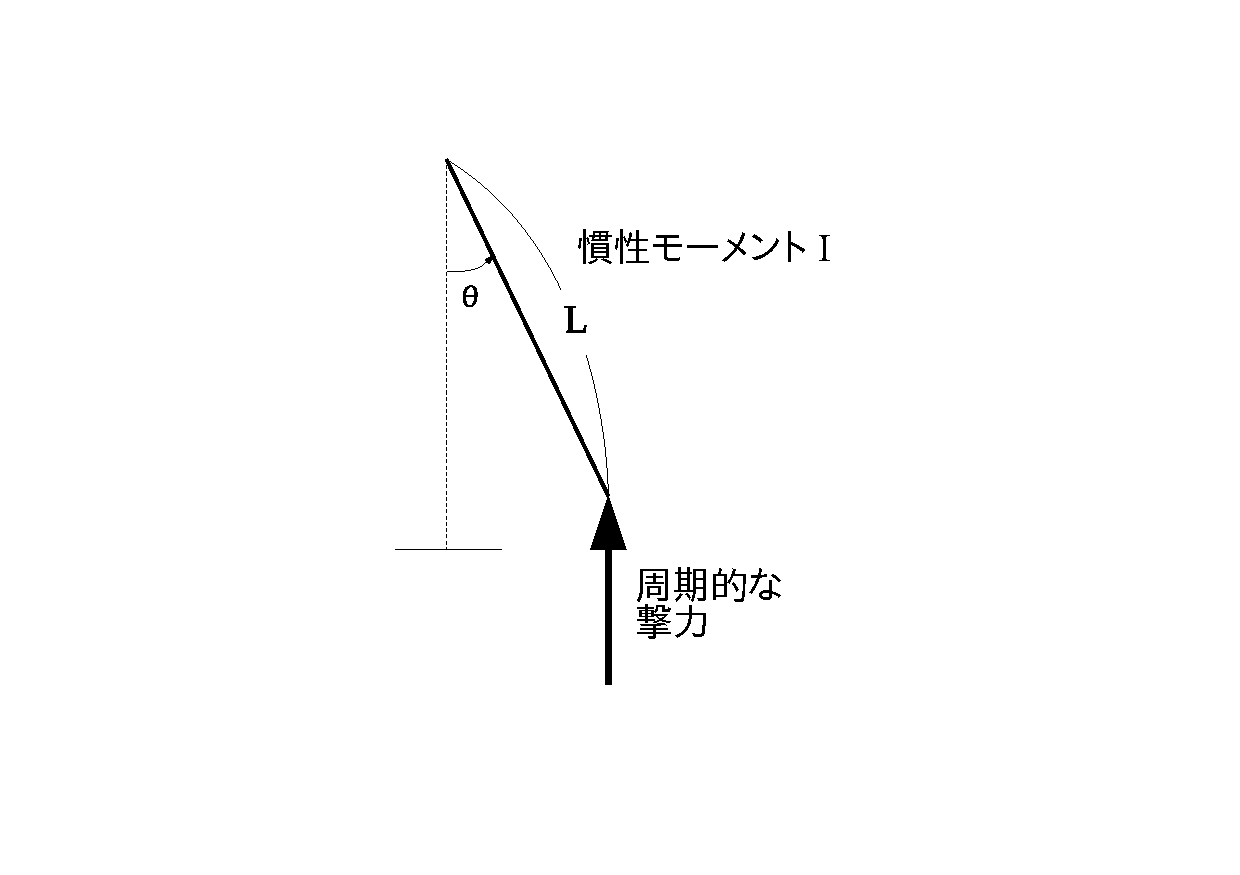
\includegraphics[width=12.5cm]{figure_1.pdf}
                \caption{撃力が加えられた慣性モーメント$I$の棒からなる回転子。重力と支点での摩擦は無視する。}
                \label{fig:f1}
            \end{center}
        \end{figure}

        
        
        式(\ref{eq:s1}),(\ref{eq:s2})の反復計算を行う前に、これらがハミルトン系、つまり$n$を大きくしていっても$q$-$p$空間における面積が一定であることを確かめておく(ここでは$q$は$\theta$を指している)。長さ$dq_{n}$と$dp_{n}$の長方形から始めることを考えると、1回の反復の後、この長方形は$dq_{n+1}$と$dp_{n+1}$の辺を持つ平行四辺形に変形される。すなわち、
        \begin{equation}
            dq_{n+1} = dq_{n} + dp_{n}
            \label{eq:e3}
        \end{equation}
        \begin{equation}
            dp_{n+1} = dp_{n} + k \cos q_{n+1} dq_{n+1}
            \label{eq:e4}
        \end{equation}

        である。式(\ref{eq:e3})に(\ref{eq:e4})を代入すると、
        \begin{equation}
            dp_{n+1} = (1 + k \cos q_{n+1})dp_{n} + k\cos q_{n+1} dq_{n}
        \end{equation}
        
        を得る。ベクトル$d\mbox{\boldmath$q$}_{n+1} = (dq_{n}, dp_{n})$と$d\mbox{\boldmath$p$}_{n+1} = (1 + k\cos q_{n}, k\cos q_{n} dq_{n}))$のベクトル積の大きさを計算して平行四辺形の面積を求めると、$dq_{n}dp_{n}$となり、位相空間内の面積は不変であり、標準写像は保存系であることがわかる。
        標準写像の定性的性質については問題6.16で調べることであるが、それらは次のように要約することができる。$k=0$のとき、棒は運動量$p_{n} = p_{0} = 一定$によって定まる一定の角運動量で回転する。$p_{0}$が$2\pi$の有理数倍のときには、位相空間の軌跡は、水平な線上にある孤立した点列から構成される(共鳴トーラス)。$p_{0}$が$2\pi$の有理数倍でないか、コンピュータに十分な精度がないときには、十分に長い時間の後に軌跡は位相空間内の水平な曲線へと変化する。そして共有トーラスに対応する孤立した点列は閉曲線へと変化する。初期条件によっては、過渡的な振る舞いが消えるくらいに十分長い反復の後に、軌跡はカオス的になるだろう。
    \section{作成したプログラム}
        本シミュレーションで作成・使用したプログラムを以下に示す。
    
    
        \subsection{パラメータの設定ウィンドウ(SetParameter.py)}
            問題6.14で使用したものと同じである。
            \listinginput{1}{SetParameter.py}
        
        \subsection{標準写像の計算・描画プログラム(6-16\_standard\_map.py)}
            このプログラムでは、初めのntransient回の計算結果を捨てて、nplot回の反復計算の結果をグラフに表示するプログラムである。プログラムを実行すると、SetParameterのshow\_setting\_windowが呼び出され、パラメータの設定が行える。OKボタンを押すと、関数staticを介してパラメータの代入とグラフの描画を行う。ここでのカウンタはscatterメソッドが標準で色のループを行わないため、自前で色の制御を行うために追加したものである。実際に写像の計算を行っているのは50行目から63行目であり、あとはグラフの体裁を整えるためのものである。
            \listinginput{1}{6-16_standard_map.py}
        
            
    \section{実習課題}
    
        \begin{enumerate}
            \renewcommand{\labelenumi}{\alph{enumi}.}
            \renewcommand{\labelenumii}{}
            
            \item 標準写像の反復を実行するプログラムを書いて、位相空間の軌跡を描け。$k$を変えたときの挙動を調べよ。特に、位相空間内の軌道の変化に着目せよ。
                \begin{enumerate}
                    \item まず、単純な問題として$k=0$として固定したとき、初期条件$p_{0}$の値をさまざまに変えたときの軌跡の様子を図\ref{fig:f2}に示す。この図は、周期的な撃力がないときには、棒は初めの角運動量を保ったまま回転を続けるという事実を再現している。
                    \begin{figure}[H]
                        \begin{center}
                            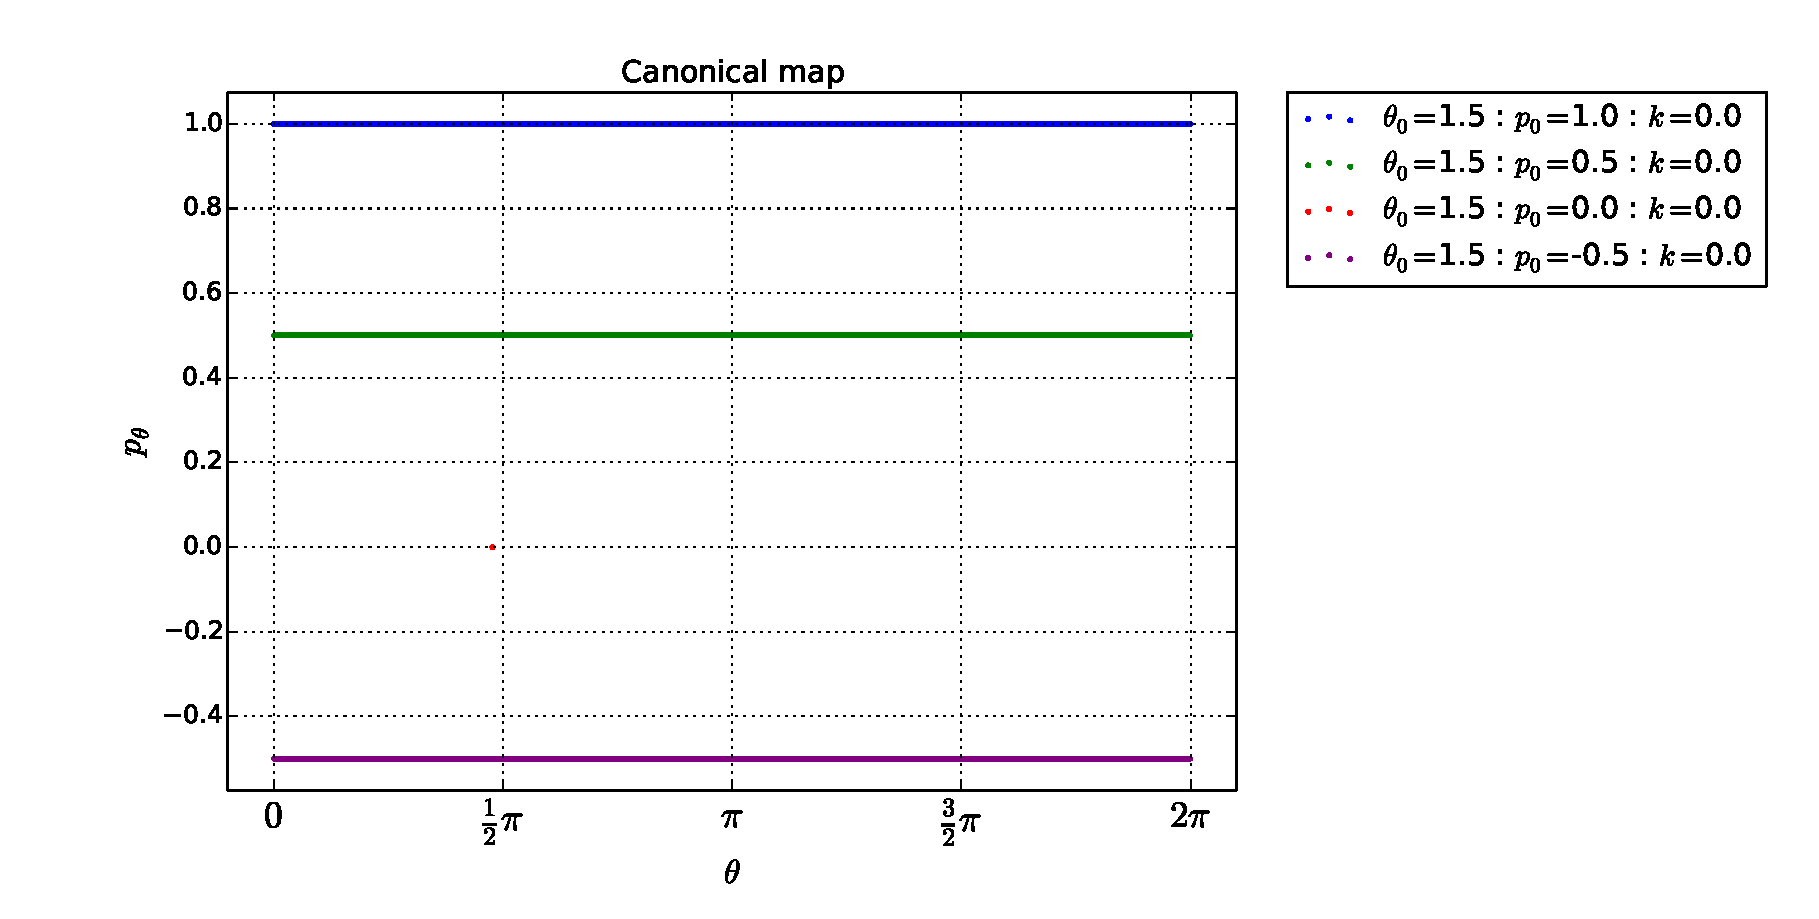
\includegraphics[width=16.5cm]{figure_2.pdf}
                            \caption{$k=0$のときの位相空間の軌跡}
                            \label{fig:f2}
                        \end{center}
                    \end{figure}
                        
                    次に、$\theta_{0}$と$p_{0}$を固定して、$k$を$k=0.1, 1.0, 1.7, 1.99694994, 1.99694995, 2.0$としたときの位相空間の軌跡を図\ref{fig:f3}、\ref{fig:f4}に示す。このグラフから、$k$が大きくなるにつれて曲線や閉曲線であった軌跡が分岐していくようになり、トーラスの島と呼ばれる環状の軌跡が現れる様子も観察される。また、$k$がある値$k=k_{c} \simeq 1.99694995$以上になると、その曲線からさらに離れた位置を取るようになって、カオス的な振る舞いを示すことも分かる。この$k_{c}$の値は、初期値によって変わることも確かめることができた。
                    \begin{figure}[H]
                        \begin{center}
                            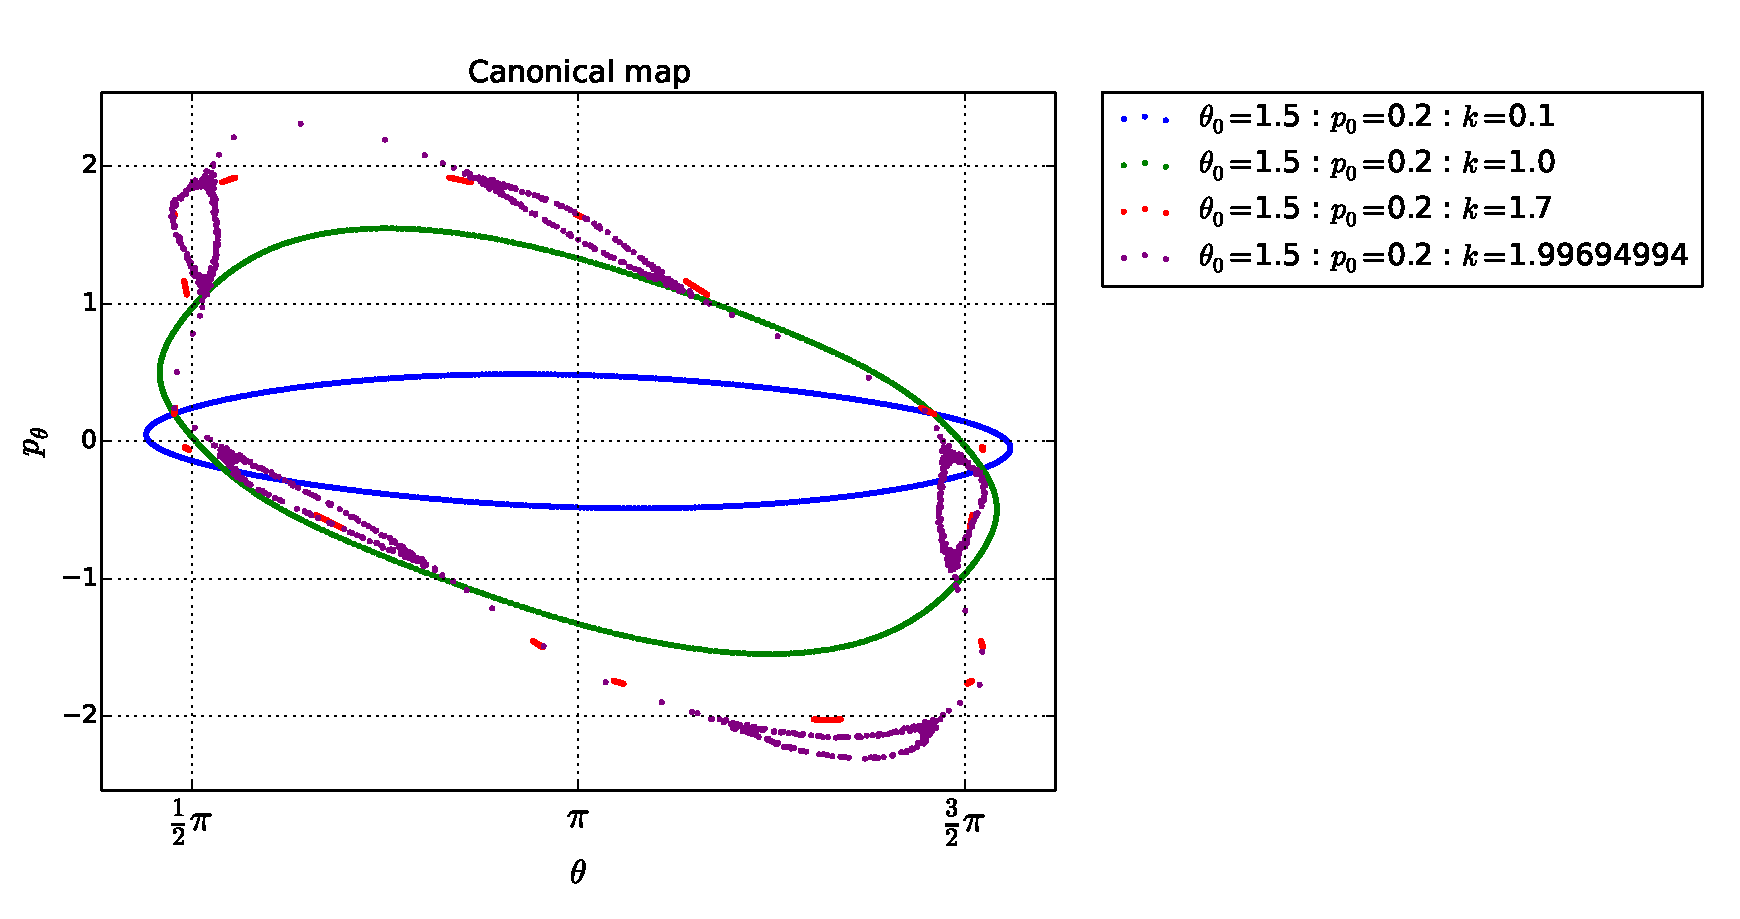
\includegraphics[width=16.5cm]{figure_3.pdf}
                            \caption{$\theta_{0}=1.5$、$p_{0}=0.2$としたとき、$k$による位相空間での軌跡の変化}
                            \label{fig:f3}
                        \end{center}
                    \end{figure}
                    
                    \begin{figure}[H]
                        \begin{center}
                            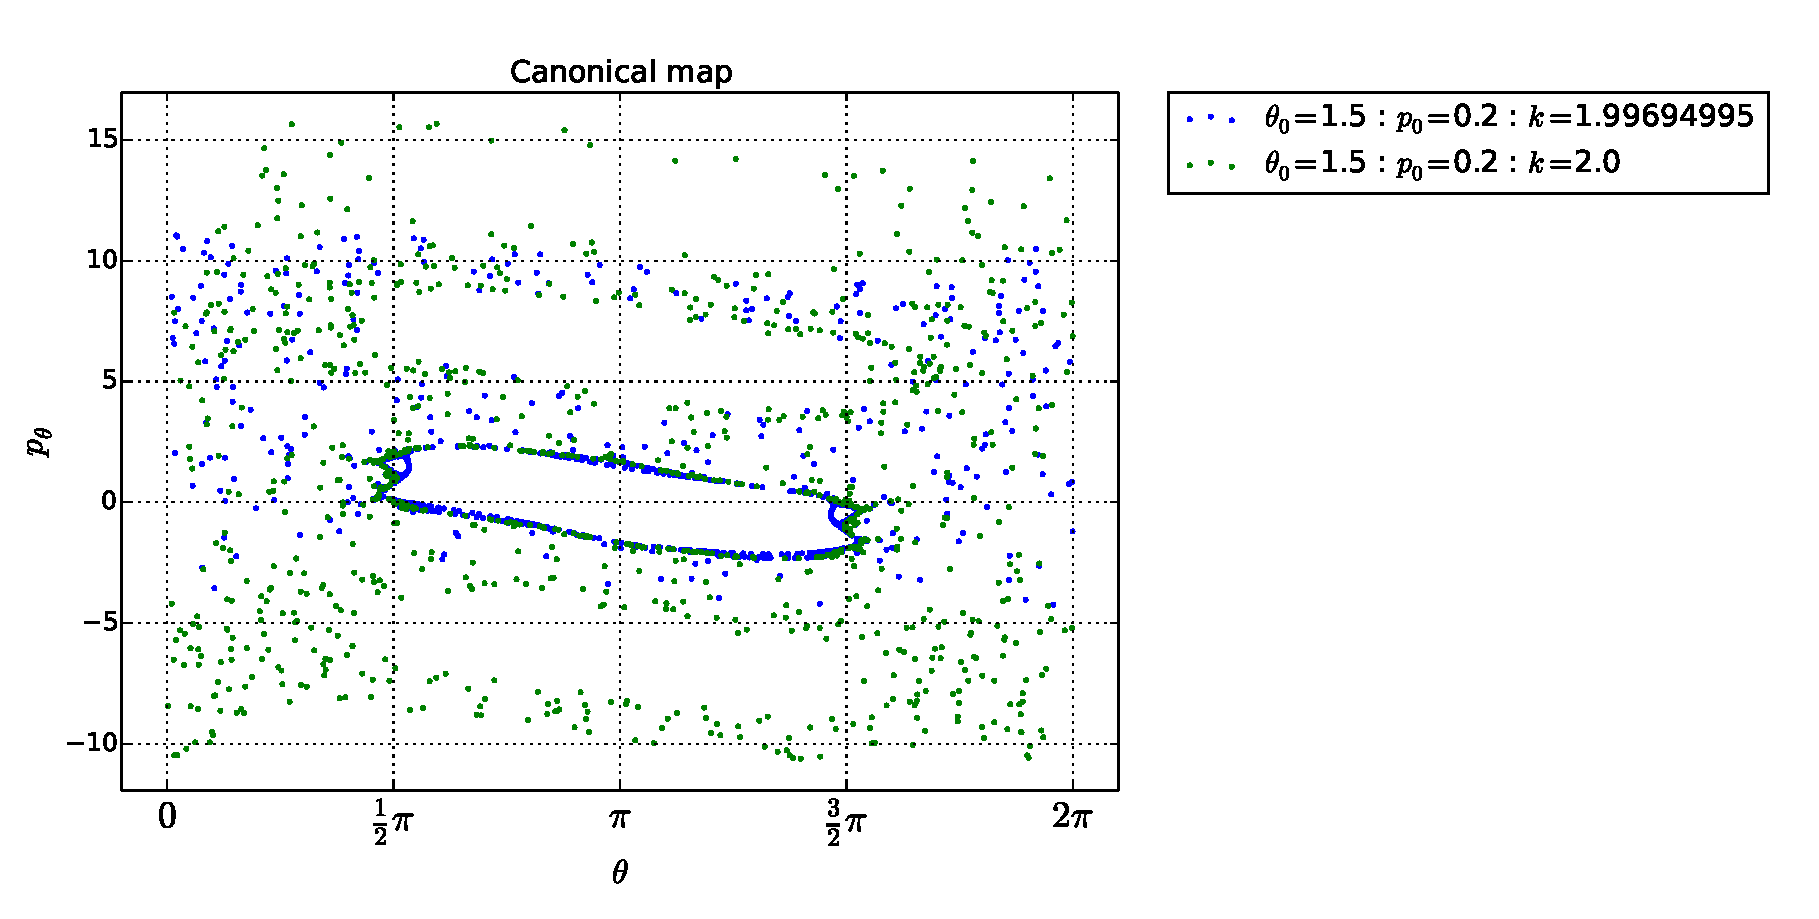
\includegraphics[width=16.5cm]{figure_4.pdf}
                            \caption{$\theta_{0}=1.5$、$p_{0}=0.2$としたとき、$k$による位相空間での軌跡の変化}
                            \label{fig:f4}
                        \end{center}
                    \end{figure}
                    
                \end{enumerate}    
            
        \end{enumerate}
    
    \section{まとめ}
        ハミルトン系の単純な例である標準写像について、$k$による位相空間での軌跡の変化を観察することができた。
    \section{参考文献}
        \begin{itemize}
            \item ハーベイ・ゴールド,ジャン・トボチニク,石川正勝・宮島佐介訳『計算物理学入門』,ピアソン・エデュケーション, 2000.
        \end{itemize}

\end{document}
